\chapter{Конструкторский раздел}

\section{Структура программы}

В программе предусмотрены два режима работы. В режиме обучения известны метки классов. По ним подбираются веса сети, а по отдельной валидационной выборке выбирается модель для применения. Тестовые данные используются после выбора модели. В режиме классификации программе передаются новый JPEG-файл и сохранённая модель. Оба режима используют один и тот же алгоритм извлечения признаков (рисунок~\ref{fig:structure}).

\begin{figure}[htbp]
  \centering
  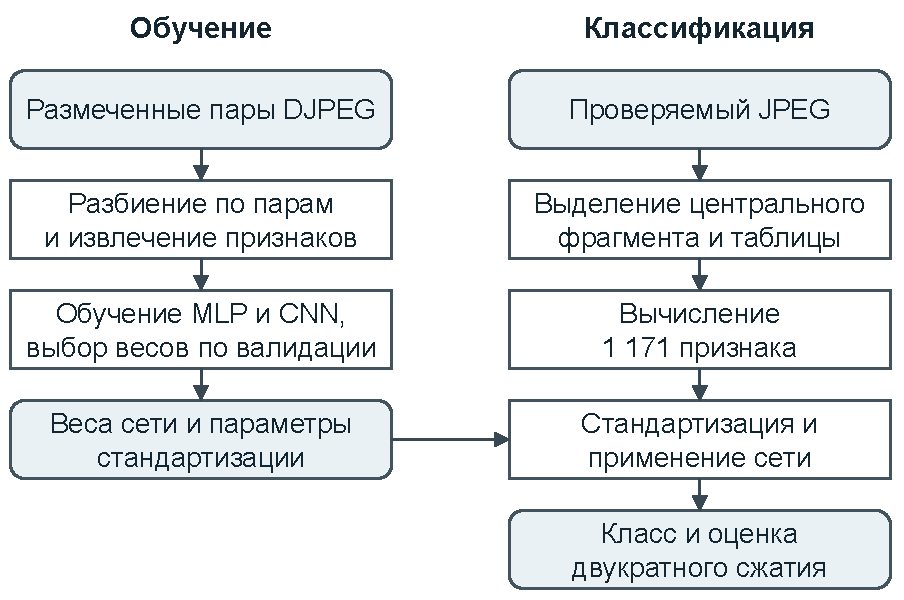
\includegraphics[width=0.86\linewidth]{images/detector-structure.drawio.pdf}
  \caption{Подготовка модели и классификация нового JPEG-файла}
  \label{fig:structure}
\end{figure}

Вместе с весами передаются статистики обучающей выборки. Благодаря этому одинаковое значение признака преобразуется одинаково при обучении и при обработке нового снимка. Для каталога модель загружается один раз, после чего каждый файл проходит ту же обработку, что и при одиночном запуске.

\section{Подготовка размеченных данных}

В наборе DJPEG фрагменту исходного снимка соответствуют два файла с общим идентификатором. Один файл получен после первого сохранения, другой --- после второго~\cite{park2018,djpeg_dataset}. Единицей разбиения служит пара. Так обе версии одного фрагмента всегда остаются вместе.

Алгоритм дополнительно объединяет соседние идентификаторы фрагментов в группы по 1\,000 номеров. Сначала группы случайно распределяются между обучающей, валидационной и тестовой частями. Затем внутри каждой части выбираются полные пары. В итоговом списке сохраняются путь, класс, номер фрагмента и принадлежность к выборке. Для отделения точных копий используются контрольные суммы декодированных пикселей. В архиве отсутствуют идентификаторы полноразмерных фотографий. Разные фрагменты одного снимка могут оказаться в разных выборках.

\section{Извлечение признаков}

Пусть ширина и высота снимка равны $W$ и $H$ пикселям. Из яркостной компоненты выделяется фрагмент $256\times256$ с координатами левого верхнего угла
\begin{equation}
  x_0=8\left\lfloor\frac{W-256}{16}\right\rfloor,\qquad
  y_0=8\left\lfloor\frac{H-256}{16}\right\rfloor.
  \label{eq:crop}
\end{equation}
Такое округление смещает границу центрального фрагмента к ближайшей предшествующей границе блока. Масштаб изображения сохраняется.

Фрагмент содержит $32\times32=1\,024$ блока размером $8\times8$. Из яркости каждого отсчёта вычитается 128, затем для каждого блока вычисляется двумерное ортонормированное ДКП. Используются первые девять переменных составляющих при зигзагообразном обходе матрицы коэффициентов. Для каждой из девяти позиций собираются значения из всех 1\,024~блоков. Постоянная составляющая $(0,0)$ в признаки не входит.

Каждое значение $c$ заменяется целым числом $\lfloor c+0{,}5\rfloor$. Для чисел от $-60$ до~60 предусмотрен отдельный интервал гистограммы. Ещё два интервала собирают значения ниже и выше этих границ. Число отсчётов в каждом интервале делится на 1\,024. Сумма 123 относительных частот одной гистограммы равна единице. Коэффициенты здесь рассчитаны по декодированным пикселям, поэтому при построении гистограммы учитывается и округление яркости при декодировании JPEG.

Девять гистограмм дают $9\times123=1\,107$~признаков. К ним добавляются 64~шага из таблицы квантования яркости, каждый делится на 255. Для каждого из $1\,171$ признаков применяется стандартизация по формуле
\begin{equation}
 \widetilde{x}_j =
 \frac{x_j-\mu_j}{\max(\sigma_j,\,1/1\,024)}.
 \label{eq:scale}
\end{equation}
Здесь $\mu_j$ и $\sigma_j$ --- среднее и стандартное отклонение признака~$j$ по обучающей выборке. Нижняя граница знаменателя равна вкладу одного блока в гистограмму и ограничивает усиление редких признаков.

\section{Архитектуры и обучение моделей}

Персептрон принимает весь вектор из 1\,171~значения. Его скрытые полносвязные слои содержат 64 и 32~нейрона. После каждого скрытого слоя применяется функция $\operatorname{ReLU}(z)=\max(0,z)$. Выходной слой формирует два числа --- оценки до нормировки для класса~0 и класса~1. Персептрон имеет 77\,154 обучаемых параметра.

В свёрточной сети гистограммы образуют девять входных каналов. Фильтр перемещается вдоль оси интервалов, поэтому один и тот же набор весов может обнаружить локальный пик в нескольких частях распределения. Длины ядер двух свёрток равны 5 и~3, число выходных каналов --- 16 и~32. Дополнение нулями сохраняет длину оси интервалов после каждой свёртки. За функцией ReLU следует усреднение соседних отсчётов с окном и шагом~2. Длина уменьшается со 123 до~61, затем до~30.

\begin{figure}[htbp]
  \centering
  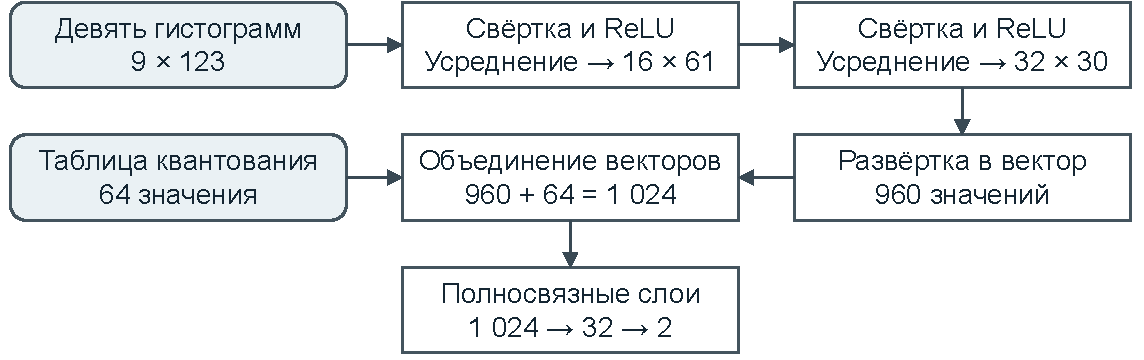
\includegraphics[width=0.98\linewidth]{images/histogram-cnn.drawio.pdf}
  \caption{Преобразование гистограмм и присоединение таблицы квантования в CNN}
  \label{fig:cnn}
\end{figure}

Как показано на рисунке~\ref{fig:cnn}, свёрточная ветвь даёт $32\times30=960$ значений. Вместе с 64~элементами таблицы квантования они поступают на полносвязный слой из 32~нейронов с функцией ReLU. Выходной слой, как и у MLP, содержит два нейрона. Всего в CNN 35\,170 обучаемых параметров.

Пусть $p_{i,y_i}$ --- оценка, которую сеть после нормировки softmax присвоила истинному классу $y_i$ для примера~$i$. Обе сети обучаются по кросс-энтропии. Для пакета из $m$ примеров функция потерь имеет вид
\begin{equation}
 L=-\frac{1}{m}\sum_{i=1}^{m}\ln p_{i,y_i}.
 \label{eq:loss}
\end{equation}
Чем меньше оценка истинного класса, тем больше вклад примера в потери.

Перед каждой эпохой примеры перемешиваются. Для очередного пакета градиенты функции~\eqref{eq:loss} вычисляются обратным распространением ошибки, затем алгоритм Adam обновляет веса. После эпохи потери вычисляются на валидационной выборке. Если значение стало меньше предыдущего минимума, сохраняются текущие веса. Обучение завершается по достижении предельного числа эпох или после заданного числа эпох без улучшения. Для каждой архитектуры выбирается запуск с минимальной валидационной потерей. То же правило определяет модель для программы.

\section{Классификация изображения}

Пусть $z_0$ и $z_1$ --- выходные значения выбранной сети. Оценка класса двукратного сжатия $s$ вычисляется функцией softmax по формуле
\begin{equation}
 s=\frac{\exp z_1}{\exp z_0+\exp z_1}.
 \label{eq:softmax}
\end{equation}
При $s\geqslant0{,}5$ программа выдаёт класс~1, иначе --- класс~0. Значение $s$ позволяет упорядочить результаты для ручного просмотра. Для неподдерживаемого файла класс и оценка не вычисляются.

\subsection*{Выводы}
Единый алгоритм формирует для обеих сетей девять гистограмм и таблицу квантования. Различие состоит в том, как сети используют соседство интервалов. Пары фрагментов распределяются между выборками до обучения, а параметры стандартизации и веса сохраняются для последующей классификации.
